\documentclass[english]{beamer}

\mode<presentation> {
  \usetheme{Warsaw}
}
\usepackage{algorithm2e}
\usepackage[english]{babel}
\usepackage[utf8]{inputenc}
\usepackage{times}
\usepackage[T1]{fontenc}
\usepackage{hyperref}
\usepackage{yhmath} %pour la commande \widering (intérieur topologique)

\DeclareMathOperator*{\argmin}{argmin}
\DeclareMathOperator*{\argmax}{argmax}
\DeclareMathOperator*{\sup2}{sup}
\DeclareMathOperator*{\inf2}{inf}
\DeclareMathOperator*{\max2}{max}
\DeclareMathOperator*{\min2}{min}


\newcommand{\Max}{\mathop{\mathrm{Max}}}
\newcommand{\R}{\mathbb{R}}
\newcommand{\Z}{\mathbb{Z}}
\newcommand{\E}{\mathbb{E}}
\newcommand{\xx}{\mathbf{x}}
\newcommand{\yy}{\mathbf{y}}
\newcommand{\zz}{\mathbf{z}}
\newcommand{\bxi}{\boldsymbol{\xi}}
\newcommand{\nyq}{\boldsymbol{\eta}}
\newcommand{\tv}{\mathrm{TV}}
\newcommand{\si}{\mathrm{SI}}
\newcommand{\m}{\mathrm{m}}
\newcommand{\num}{\mathrm{num}}
\newcommand{\denom}{\mathrm{denom}}
\renewcommand{\v}{\mathrm{v}}
\newcommand{\gpc}{\mathrm{GPC}}
\renewcommand{\P}{\mathbb{P}}
\newcommand{\var}{\mathbb{V}\mathrm{ar}}
\newcommand{\sgn}{\mathrm{sgn}}
\renewcommand{\widering}[1]{\ring{\wideparen{#1}}}

\newcommand{\RR}{\mathbb{R}}
\newcommand{\qr}{\textrm{QsRank}}

\theoremstyle{plain}
\newtheorem{theoreme}{Th\'eor\`eme}[section]
\newtheorem{algo}{Algorithme}[section]
\newtheorem{lemme}[theoreme]{Lemme}
\newtheorem{proposition}[theoreme]{Proposition}
\newtheorem{corollaire}[theoreme]{Corollaire}
\theoremstyle{remark}
\newtheorem{exemple}{Exemple}[section]

\hypersetup{
      pdfpagemode = FullScreen,% afficher le pdf en plein écran
      pdfauthor   = {Arthur Darcet \& Yohann Salaun},%
      pdftitle    = {Qs Rank and efficient $\epsilon$-neighbor search},%
      pdfsubject  = {MVA},%
      pdfcreator  = {PDFLaTeX},%
      pdfproducer = {PDFLaTeX}%
}


\title[Qs Rank and efficient $\epsilon$-neighbor search]{Qs Rank and efficient $\epsilon$-neighbor search}

%\subtitle {à partir de l'article \\ ``An explicit sharpness index \\ related to global phase coherence'' \\ 
%																			de G. Blanchet et L. Moisan}

\author[Arthur Darcet \& Yohann Salaun] 
{Arthur Darcet \& Yohann Salaun}

\addtobeamertemplate{footline}{\insertframenumber/\inserttotalframenumber} %numéroter des slides

\begin{document}

\begin{frame}
  \titlepage
\end{frame}

\begin{frame}{Summary}
  \tableofcontents
\end{frame}

%%%%%%%%%%%%%%%%%%%%%%%%%%% Fin de l'en-tete %%%%%%%%%%%%%%%%%%%%%%%%%%%%

\section{Introduction}

\begin{frame}{Introduction}
\begin{figure}[htbp]
	\begin{center}
	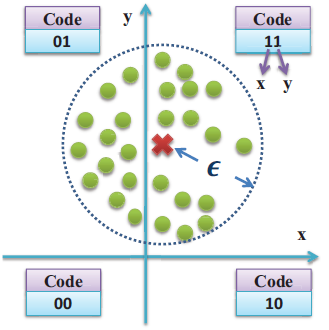
\includegraphics[width=.4\linewidth]{Images/intro.png}
	\caption{$\epsilon$-neighbor search}
	\end{center}
	\label{fig:intro}
\end{figure}
\emph{QsRank: Query-sensitive Hash Code Ranking for Efficient Epsilon-neighbor Search}, CVPR 2012

\end{frame}

\section{Theoretical Description}

\subsection{Hash Codes}

\begin{frame}{Hash Codes}

\begin{figure}[htbp]
	\begin{center}
	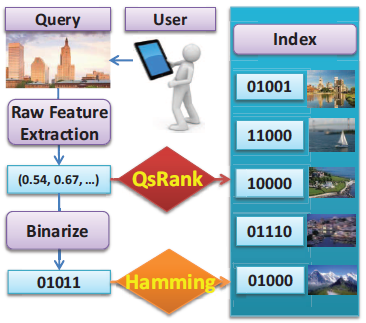
\includegraphics[width=.5\linewidth]{Images/intro2.png}
	\caption{data binarization}
	\end{center}
	\label{fig:intro2}
\end{figure}
\begin{itemize}
	\item[\textbf{1.}] Hash code generation of the data for faster retrieval
	\item[\textbf{2.}] Ranking of the hash code depending on a query
\end{itemize}

\end{frame}

\begin{frame}{Hash Codes generation}
\textbf{Principal Component Analysis:}\\
\vspace{1em}
$\forall j \in [1;d],\ h_j = $	
\begin{itemize}
    \item[$\bullet$]1 $\text{ if }(PCA(x, \{x_i\}_i))_j > 0$
    \item[$\bullet$]0 $\text{ if }(PCA(x, \{x_i\}_i))_j \leq 0$
\end{itemize}
\vspace{1em}
\begin{itemize}
	\item[\textbf{1.}]dimension decrease but keep information
	\item[\textbf{2.}]orthogonal projection that preserves the $L^2$-norm
	\item[\textbf{3.}]uncorrelated PCA values which leads to an efficient ranking with Qs Rank.
\end{itemize}
\end{frame}

\subsection{Qs Rank}

\begin{frame}{Qs Rank Formula}
\[
	\qr(q, h, \epsilon) = \frac{\int_{NN(q,\epsilon) \cap S(h)} p(y) dy}{\int_{NN(q,\epsilon)} p(y) dy} = \mathbb{P}(y \in S(h) | y\in NN(q,\epsilon))
\]
where:
\begin{enumerate}
	\item[$\bullet$]$NN(q,\epsilon) = \{y \in \RR^d \text{ s.t. } ||y-q||<\epsilon\}$ is the $\epsilon$-ball around the query $q$
	\item[$\bullet$]$S(h) = \{y \in \RR^d \text{ s.t. } \forall i \in [1;d] y_i h_i > 0 \}$ is the set described by the hash code $h$
\end{enumerate}
\end{frame}

\begin{frame}{Qs Rank Approximations}
\[
	\begin{array}{ccc}
	\qr(q, h, \epsilon) 
	& \approx & \frac{\int_{NN(q^k,\epsilon) \cap S(h^k)} p(y^k) dy^k}{\int_{NN(q^k,\epsilon)} p(y^k) dy^k}\\
	\pause
	& \approx & \frac{\int_{HC(q^k,\epsilon) \cap S(h^k)} p(y^k) dy^k}{\int_{HC(q^k,\epsilon)} p(y^k) dy^k}
	\end{array}
\]
where $HC(q^k,\epsilon) = \{y^k \in \RR^k \text{ s.t. } \forall i \in [1;k], |y^k_i-q^k_i|<\epsilon\}$
\end{frame}

\begin{frame}{Qs Rank Approximations}
\[
	\begin{array}{ccc}
	\qr(q, h, \epsilon) 
	& \approx & \frac{\int_{NN(q^k,\epsilon) \cap S(h^k)} p(y^k) dy^k}{\int_{NN(q^k,\epsilon)} p(y^k) dy^k}\\
	& \approx & \frac{\int_{HC(q^k,\epsilon) \cap S(h^k)} p(y^k) dy^k}{\int_{HC(q^k,\epsilon)} p(y^k) dy^k}\\
	& \approx & \prod_{i=1}^k \frac{\int_{|y^k_i - q^k_i| < \epsilon, y^k_i h^k_i > 0 } p(y^k_i) dy^k_i}{\int_{|y^k_i - q^k_i| < \epsilon} p(y^k_i) dy^k_i}
	\end{array}
\]
\end{frame}

\begin{frame}{Qs Rank Approximations}
\[
	\qr(q, h, \epsilon) \approx \prod_{i=1}^k \mathbb{P}(y^k_i \in S(h^k_i) | y^k_i \in HC(q^k_i,\epsilon))
\]
We suppose also that $y^k\sim \mathcal{U}(\RR^k)$:
\[
	\begin{array}{ccc}
	\qr(q, h, \epsilon) 
	& \approx & \prod_{i=1}^k \frac{\int_{|y^k_i - q^k_i| < \epsilon, y^k_i h^k_i > 0 } dy^k_i}{\int_{|y^k_i - q^k_i| < \epsilon} dy^k_i} \\
	& \approx & \prod_{i=1}^k \text{clamp} (\frac{1}{2}( 1 + \frac{h^k_i q^k_i}{\epsilon} ), [0;1] )                  
	\end{array}
\]
\end{frame}

\section{Retrieval Procedure}

\begin{frame}
\begin{figure}[htbp]
	\begin{center}
	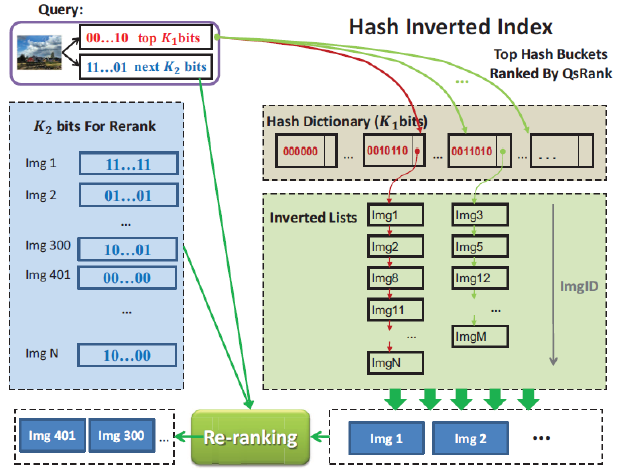
\includegraphics[width=.6\linewidth]{Images/algo.png}
	\caption{Retrieval procedure: Buckets ranking ($K_1$ bits). Neighbors re-ranking ($K_1+K_2$ bits)}
	\end{center}
	\label{fig:algo}
\end{figure}
\end{frame}

\section{Results}

\begin{frame}

\begin{figure}[htbp]
	\begin{center}
	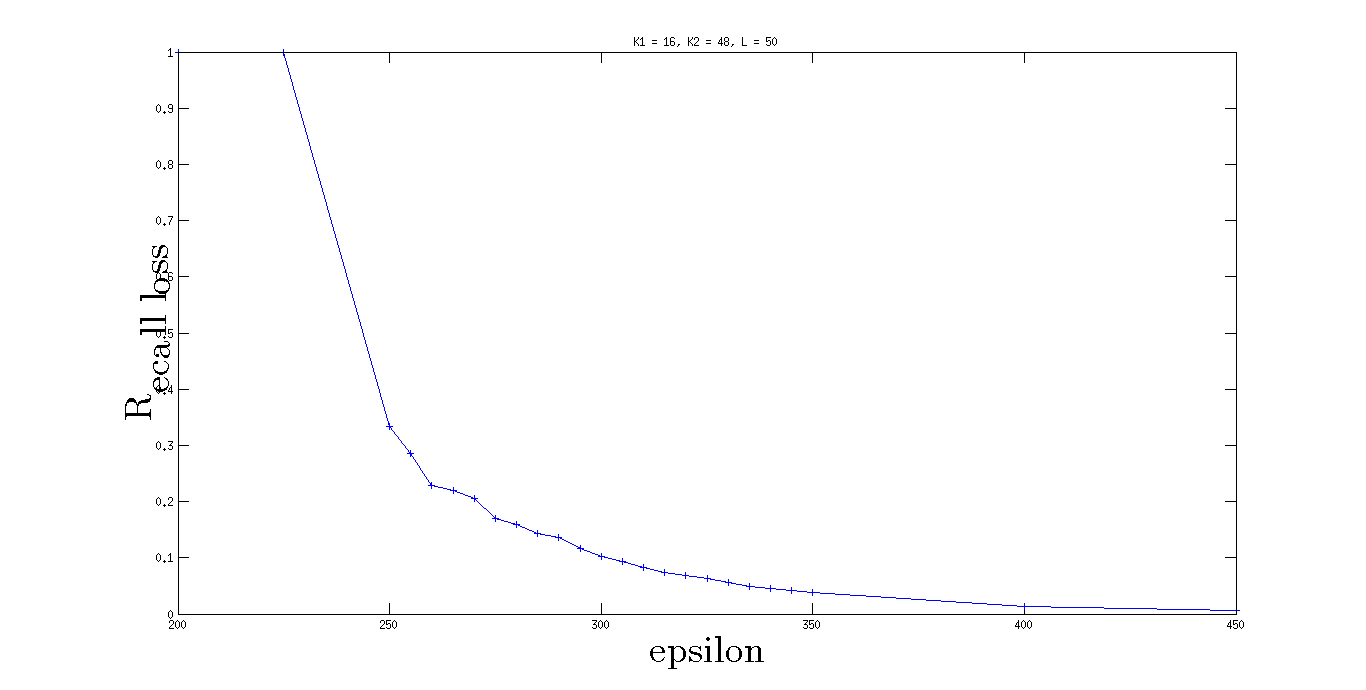
\includegraphics[width=.8\linewidth]{Images/rloss.png}
	\end{center}
	\caption{Recall Loss function of epsilon.}
	\label{fig:rloss}
\end{figure}

\end{frame}

\bibliographystyle{plain} %Style of Bibliography: plain / apalike / amsalpha / ...
\bibliography{literature} %You need a file 'literature.bib' for this.

\end{document}

